% Beamer - Exposé M1 : Autoencodeurs & Débruitage
% Compiler (au choix): pdflatex/xelatex/lualatex
\documentclass[11pt,aspectratio=169]{beamer}

% --- Langue / encodage ---
\usepackage[T1]{fontenc}
\usepackage[utf8]{inputenc}
\usepackage[french]{babel}

% --- Maths / figures ---
\usepackage{amsmath,amssymb,mathtools}
\usepackage{graphicx}
\usepackage{booktabs}
\usepackage{tikz}
\usetikzlibrary{arrows.meta,positioning,calc}
\usepackage{xcolor}
\usepackage[most]{tcolorbox}
\usepackage{xurl}
\urlstyle{same}

% --- Code (sans shell-escape, portable) ---
\usepackage{listings}
\lstset{
  basicstyle=\ttfamily\footnotesize,
  columns=fullflexible,
  breaklines=true,
  frame=single,
  showstringspaces=false
}

% --- Theme : simple, avec une couleur d'accent uniforme ---
\usetheme{Madrid}
\usecolortheme{default}
\definecolor{accent}{RGB}{0, 88, 122}
\setbeamercolor{structure}{fg=accent}
\setbeamertemplate{blocks}[rounded][shadow=true]
\setbeamercolor{block title}{bg=accent, fg=white}
\setbeamercolor{block body}{bg=accent!6, fg=black}
\setbeamercolor{block title example}{bg=accent, fg=white}
\setbeamercolor{block body example}{bg=accent!6, fg=black}
\setbeamercolor{block title alerted}{bg=accent, fg=white}
\setbeamercolor{block body alerted}{bg=accent!6, fg=black}
\setbeamertemplate{navigation symbols}{}
\setbeamertemplate{headline}{}
\setbeamertemplate{footline}{%
  \leavevmode%
  \hfill%
  \usebeamerfont{page number in head/foot}%
  \insertframenumber{} / \inserttotalframenumber\hspace{0.6em}%
  \vspace{0.3em}%
}

% --- Chemins d'images (depuis /docs) ---
\graphicspath{{../assets/figures/}{../assets/logos/}}

% --- Macros ---
\newcommand{\R}{\mathbb{R}}
\newcommand{\E}{\mathbb{E}}
\newcommand{\norm}[1]{\left\lVert #1 \right\rVert}
\newcommand{\formula}[1]{\begin{block}{Formule}#1\end{block}}
\newcommand{\accentbox}[1]{%
  \begin{center}
  \begin{tcolorbox}[
    enhanced,
    width=0.94\linewidth,
    colback=accent!6,
    colframe=accent,
    arc=2.2mm,
    boxrule=0.6pt,
    left=6pt,right=6pt,top=6pt,bottom=6pt,
    drop shadow={black!35!white}
  ]
  #1
  \end{tcolorbox}
  \end{center}
}

% --- Métadonnées ---
\title[AE \& Débruitage]{\texorpdfstring{Autoencodeurs et débruitage d'images\\(Denoising Autoencoders)}{Autoencodeurs et débruitage d'images (Denoising Autoencoders)}}
\subtitle{Master 1 Sciences et Technologies de l'Espace}
\author[Henovi \& al.]{Alban Komla Henovi \and Asta Walo Diop \and Arthur Bomemo Walé}
\institute[Traitement d'Images Optiques]{Traitement d'Images Optiques}
\date{18 avril 2026}

\titlegraphic{%
  \vspace{-0.3cm}%
  \IfFileExists{institut_logo.jpg}{\includegraphics[height=1.1cm,keepaspectratio]{institut_logo.jpg}}{}\hspace{0.6cm}%
  \IfFileExists{logo_craste-lf.png}{\includegraphics[height=1.1cm,keepaspectratio]{logo_craste-lf.png}}{}\hspace{0.6cm}%
  \IfFileExists{logo_onu.png}{\includegraphics[height=1.1cm,keepaspectratio]{logo_onu.png}}{}%
}

\begin{document}

% -----------------------------------------------------------------------------
\begin{frame}[plain]
  \vspace*{0.25cm}
  \hbox to \linewidth{%
    \IfFileExists{logo_onu.png}{\includegraphics[height=1.1cm,keepaspectratio]{logo_onu.png}}{}%
    \hspace{0.35cm}%
    \IfFileExists{logo_craste-lf.png}{\includegraphics[height=1.1cm,keepaspectratio]{logo_craste-lf.png}}{}%
    \hfil%
    \IfFileExists{institut_logo.jpg}{\includegraphics[height=1.1cm,keepaspectratio]{institut_logo.jpg}}{}%
  }

  \vspace{0.55cm}
  \centering
  \accentbox{\centering\Large\bfseries \inserttitle\par}
  \vspace{0.3cm}
  {\large \insertsubtitle\par}
  \vspace{0.45cm}
  {\normalsize \textbf{CENTRE REGIONAL AFRICAIN DES SCIENCES ET TECHNOLOGIES DE L'ESPACE}\par}
  \vspace{0.2cm}
  {\normalsize \insertauthor\par}
  \vspace{0.2cm}
  {\normalsize \insertinstitute\par}
  \vspace{0.2cm}
  {\normalsize \insertdate\par}
  \vspace{0.2cm}
\end{frame}

\begin{frame}{Plan}
  \tableofcontents
\end{frame}

% -----------------------------------------------------------------------------
\section{Contexte et objectif}

\begin{frame}{Pourquoi le débruitage en imagerie optique ?}
\begin{itemize}
  \item Les images optiques contiennent du bruit : capteur, conditions d'acquisition, compression, prétraitements, etc.
  \item Le débruitage vise à retrouver une image \emph{propre} à partir d'une observation bruitée.
  \item En apprentissage profond, on peut apprendre un opérateur $f_\theta$ qui approxime :
  $$x_{\text{clean}} \approx f_\theta\big(\tilde{x}\big)$$
  où $\tilde{x}$ est une version bruitée.
\end{itemize}
\end{frame}

\begin{frame}{Objectif de l'exposé}
\begin{itemize}
  \item Rappeler le principe des autoencodeurs (AE) : encodeur $E_\theta$ + décodeur $D_\theta$.
  \item Présenter l'autoencodeur débruiteur (DAE) : entrée bruitée, cible propre.
  \item Montrer une \textbf{démo notebook} (MNIST ou patches d'images) : ajout de bruit, entraînement, comparaison avant/après.
\end{itemize}
\end{frame}

% -----------------------------------------------------------------------------
\section{Autoencodeurs : principe}

\begin{frame}{Définition : autoencodeur}
\begin{itemize}
  \item Apprentissage \emph{auto-supervisé} (self-supervised) : la cible est construite à partir des données.
  \item AE apprend une représentation latente $z$ (bottleneck) puis reconstruit l'entrée.
\end{itemize}

\vspace{0.4em}
\begin{block}{Formalisme}
\begin{align*}
  z &= E_\theta(x), \quad z \in \R^d \\
  \hat{x} &= D_\theta(z) \\
  &= D_\theta\big(E_\theta(x)\big)
\end{align*}
\end{block}
\end{frame}

\begin{frame}{Schéma AE (encodeur → latent → décodeur)}
\centering
\IfFileExists{../assets/figures/autoencoder.png}{%
  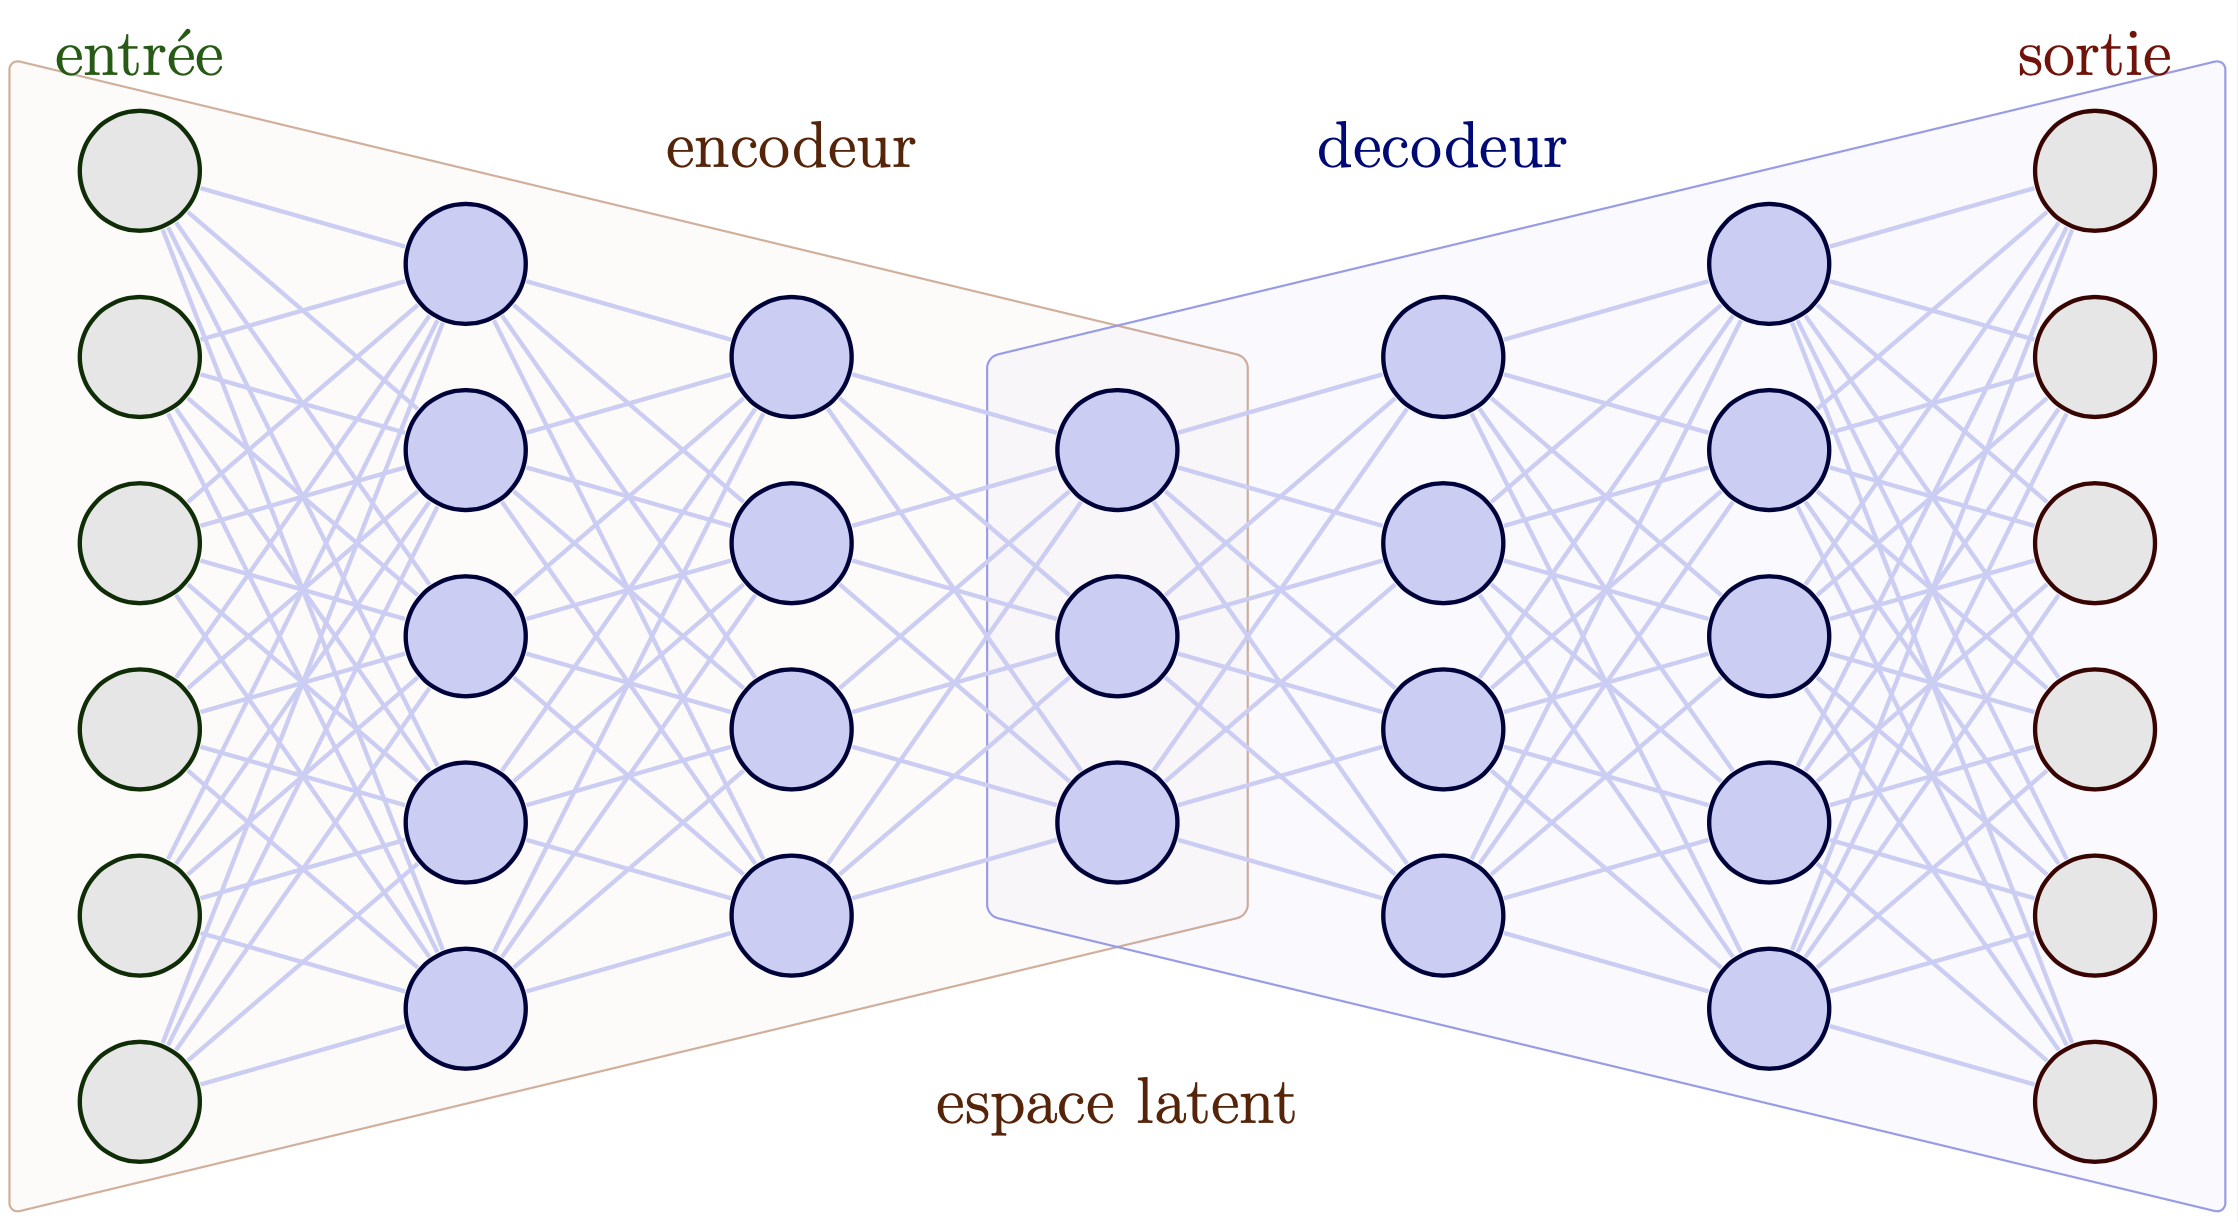
\includegraphics[width=0.95\linewidth,height=0.56\textheight,keepaspectratio]{autoencoder.png}
}{%
  \fbox{\parbox[c][0.45\textheight][c]{0.92\linewidth}{\centering \footnotesize autoencoder.png\\(absent)}}
}%

\vspace{0.6em}
\begin{itemize}
  \item Le ``goulot d'étranglement'' (dimension $d$) force une représentation compacte.
  \item Pour les images, on utilise souvent des \textbf{convolutions} (AE convolutionnel).
\end{itemize}
\end{frame}

\begin{frame}{Perte de reconstruction}
\begin{itemize}
  \item On minimise une erreur de reconstruction $\ell(x,\hat{x})$ sur un dataset de $m$ exemples.
\end{itemize}

\formula{
\[
  \mathcal{L}(\theta)=\frac{1}{m}\sum_{j=1}^m \ell\big(x^{(j)}, \hat{x}^{(j)}\big)
\]
}

\begin{exampleblock}{Exemple (images réelles) : MSE}
\[
  \ell(x,\hat{x}) = \frac{1}{N}\norm{x-\hat{x}}_2^2
\]
\end{exampleblock}
\end{frame}

% -----------------------------------------------------------------------------
\section{Autoencodeur débruiteur (DAE)}

\begin{frame}{Idée : Denoising Autoencoder}
\begin{itemize}
  \item On corrompt l'entrée $x$ via un modèle de bruit $q(\tilde{x}\mid x)$.
  \item Pour enlever du bruit, on entraîne le réseau à prédire l'image propre $x$ à partir de l'image bruitée $\tilde{x}$.
  \item En entraînement : \textbf{entrée} = images bruitées, \textbf{sortie / cible} = images originales.
\end{itemize}

\formula{
\[
  \min_\theta\; \E_{x\sim p_{\text{data}}}\; \E_{\tilde{x}\sim q(\cdot\mid x)}\; \ell\big(x,\, D_\theta(E_\theta(\tilde{x}))\big)
\]
}
\end{frame}

\begin{frame}{Schéma DAE (entrée bruitée → sortie propre)}
\centering
\IfFileExists{../assets/figures/autoencoder-denoising.png}{%
  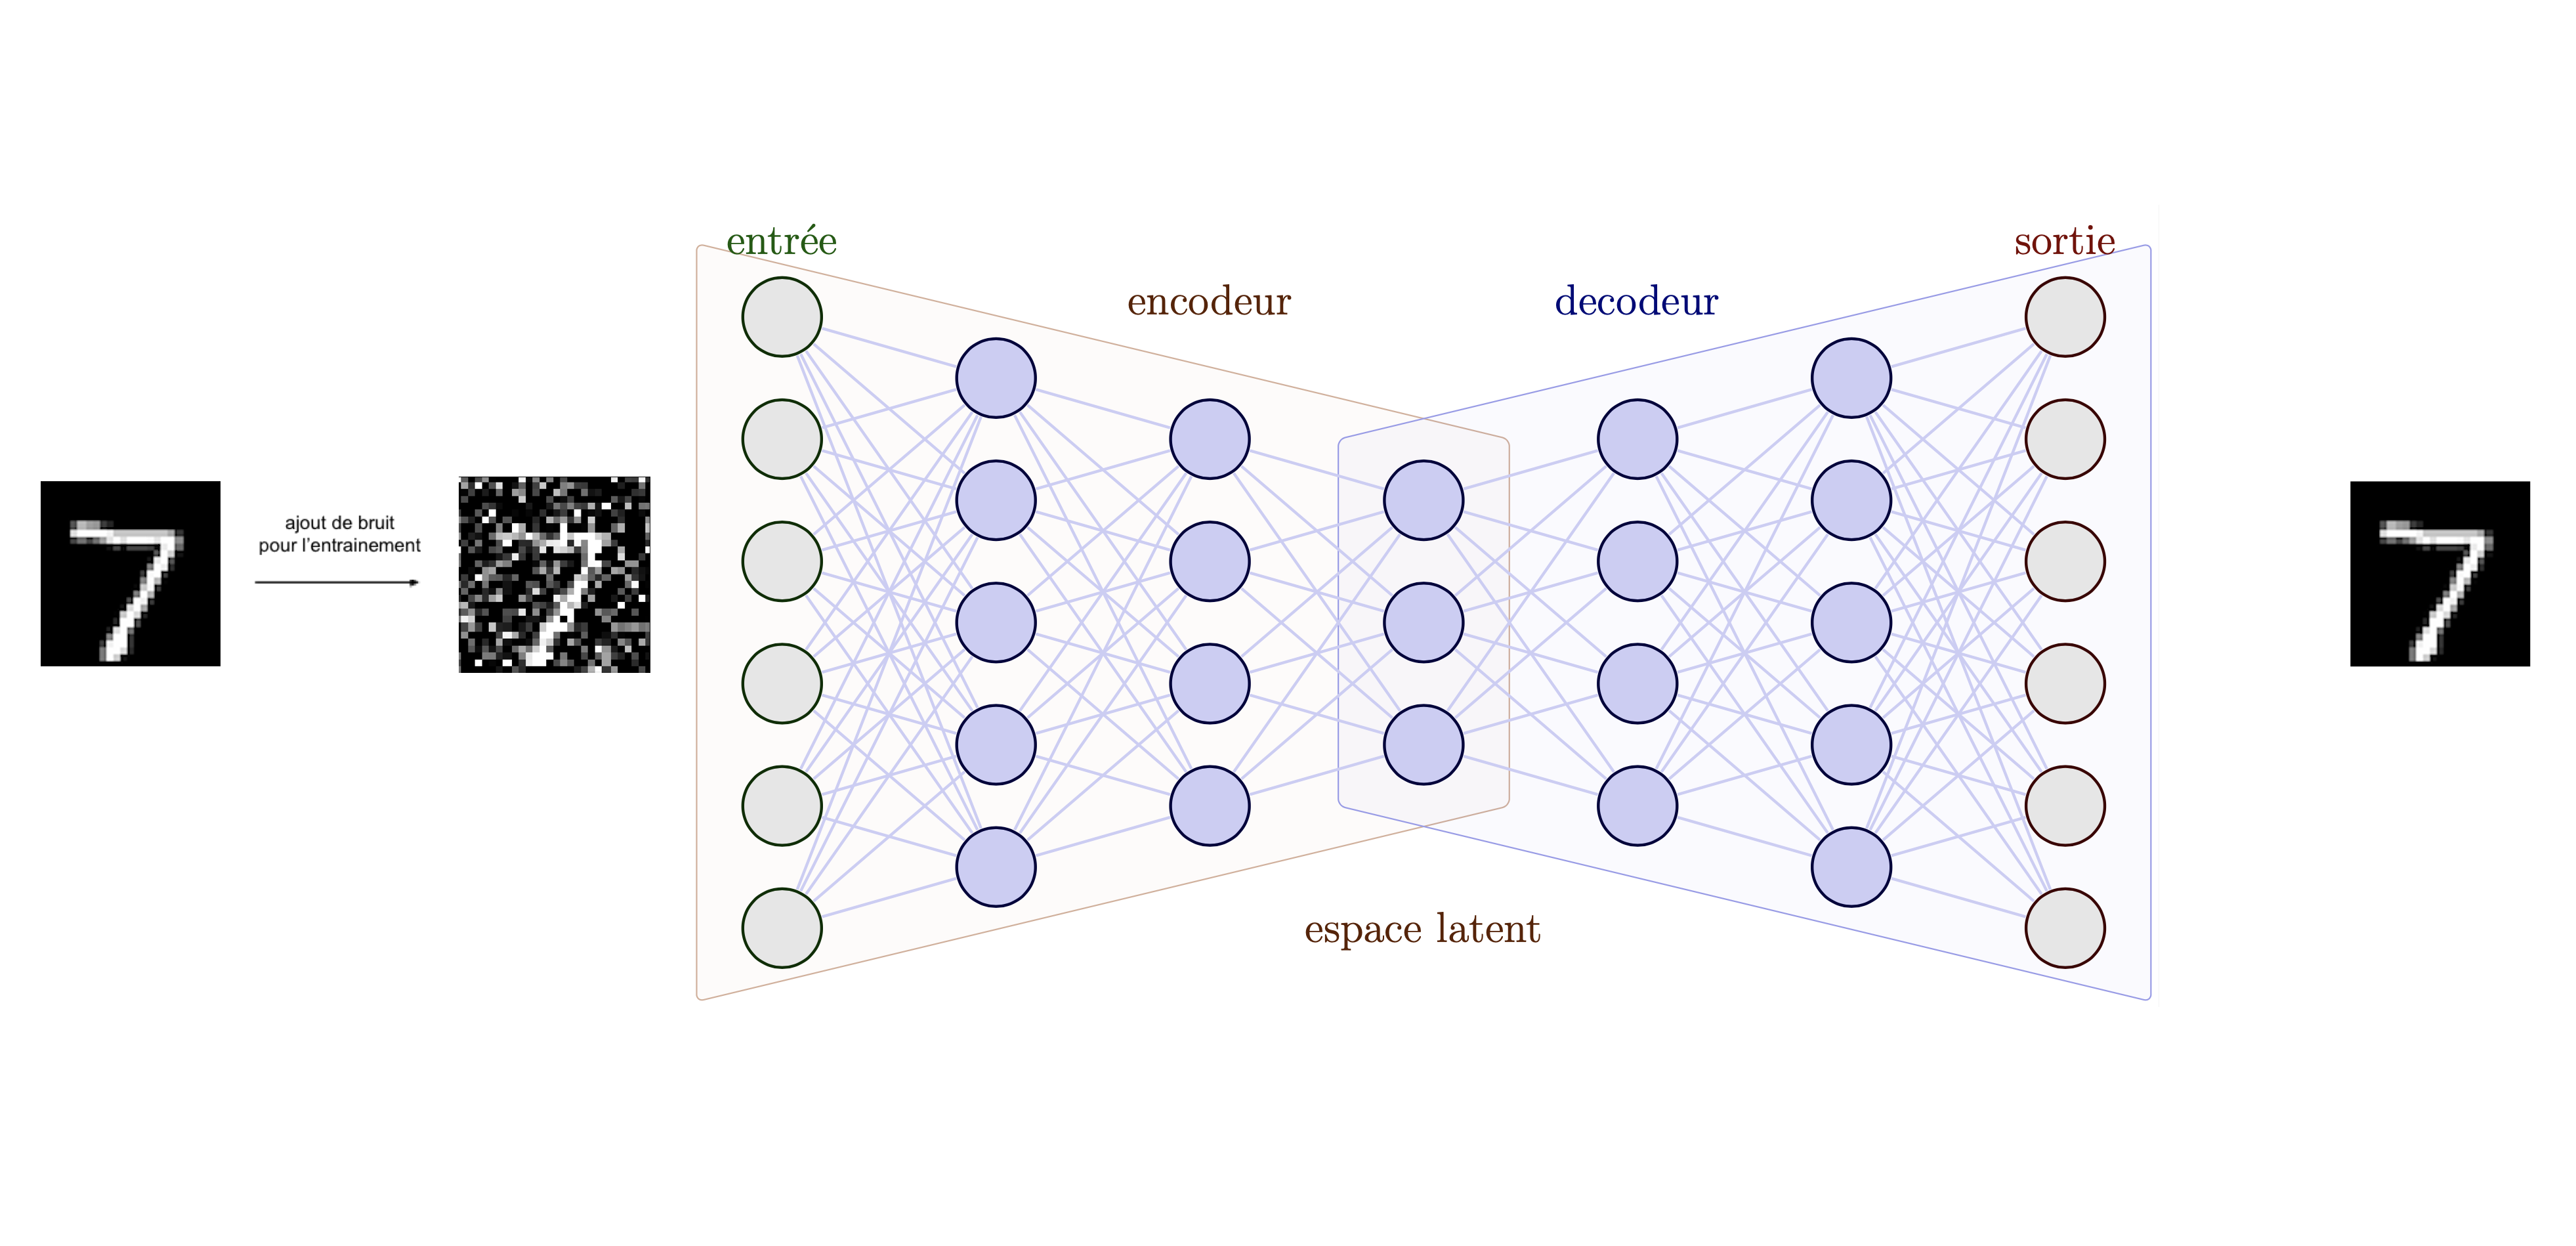
\includegraphics[width=0.95\linewidth,height=0.56\textheight,keepaspectratio]{autoencoder-denoising.png}
}{%
  \fbox{\parbox[c][0.45\textheight][c]{0.92\linewidth}{\centering \footnotesize autoencoder-denoising.png\\(absent)}}
}%

\vspace{0.6em}
\begin{itemize}
  \item Important : la distribution de bruit utilisée à l'entraînement doit être cohérente avec le bruit réel.
\end{itemize}
\end{frame}

\begin{frame}{Modèles de bruit (exemples)}
\begin{itemize}
  \item Bruit gaussien additif : $\tilde{x} = x + \sigma\,\varepsilon$, avec $\varepsilon\sim\mathcal{N}(0,I)$.
  \item Bruit impulsionnel (``sel et poivre'') : pixels remplacés aléatoirement.
  \item Bruit multiplicatif (ex. speckle) : $\tilde{x}=x\odot(1+\varepsilon)$.
\end{itemize}

\begin{block}{Remarque}
Dans la démo de cette présentation, on utilise un bruit gaussien additif sur une image locale (\texttt{image1.webp}) pour illustrer l'entraînement d'un autoencodeur débruiteur.
\end{block}
\end{frame}

% -----------------------------------------------------------------------------
\section{Architecture : AE convolutionnel}

\begin{frame}{Pourquoi des convolutions ?}
\begin{itemize}
  \item Les images ont une structure spatiale : localité, invariances.
  \item Les couches convolutives réduisent le nombre de paramètres vs fully-connected.
  \item Encodeur : convolutions + pooling (réduction spatiale) ; décodeur : upsampling / conv transpose.
\end{itemize}
\end{frame}

\begin{frame}[fragile]{Pseudo-code (idée entraînement DAE)}
\begin{lstlisting}[language=Python]
for epoch in range(E):
  for x in dataloader:            # x : image propre
    x_tilde = add_noise(x)        # corruption
    x_hat = model(x_tilde)        # reconstruction
    loss = mse(x_hat, x)          # cible = propre
    loss.backward(); optimizer.step()
\end{lstlisting}

\begin{itemize}
  \item On peut évaluer sur des niveaux de bruit \emph{non vus} à l'entraînement.
\end{itemize}
\end{frame}

% -----------------------------------------------------------------------------
\section{Évaluation et métriques}

\begin{frame}{MSE, PSNR, SSIM (rappel)}
\begin{itemize}
  \item \textbf{MSE} : erreur moyenne quadratique, simple mais pas toujours perceptuelle.
  \item \textbf{PSNR} : mesure en dB, dérivée de la MSE.
\end{itemize}

\begin{block}{PSNR}
Si l'image est dans $[0,1]$, $MAX_I=1$ :
\[
\mathrm{PSNR}(x,\hat{x}) = 10\log_{10}\Big(\frac{MAX_I^2}{\mathrm{MSE}(x,\hat{x})}\Big)
\]
\end{block}

\begin{itemize}
  \item \textbf{SSIM} : mesure structurale (souvent plus corrélée à la perception).
\end{itemize}
\end{frame}

% -----------------------------------------------------------------------------
\section{Démo notebook}

\begin{frame}{Démo : déroulé (Notebook)}
\begin{enumerate}
  \item Charger l'image locale \texttt{assets/inputs/image1.webp} et normaliser dans $[0,1]$.
  \item Ajouter du bruit gaussien : $\tilde{x} = x + \sigma\varepsilon$ puis \texttt{clip} dans $[0,1]$.
  \item Extraire des \textbf{patchs} alignés (bruité/propre) pour obtenir un jeu d'entraînement.
  \item Définir un AE convolutionnel (encodeur/décodeur) et entraîner avec une perte MSE : entrée $\tilde{p}$, cible $p$.
  \item Appliquer le réseau à l'image entière et visualiser : \textbf{bruitée} vs \textbf{débruitée} vs \textbf{propre}.
\end{enumerate}
\end{frame}

\begin{frame}{Résultats sur image locale (exports du notebook)}
\begin{columns}[T,onlytextwidth]
  \column{0.33\textwidth}
  \centering
  \textbf{Entrée bruitée}\\[0.4em]
  \IfFileExists{../assets/figures/demo_noisy.png}{%
    \includegraphics[width=\linewidth]{demo_noisy.png}\\
  }{%
    \fbox{\parbox[c][0.45\textheight][c]{0.92\linewidth}{\centering \footnotesize demo\_noisy.png\\(absent)}}\\
  }%

  \column{0.33\textwidth}
  \centering
  \textbf{Sortie AE}\\[0.4em]
  \IfFileExists{../assets/figures/demo_denoised.png}{%
    \includegraphics[width=\linewidth]{demo_denoised.png}\\
  }{%
    \fbox{\parbox[c][0.45\textheight][c]{0.92\linewidth}{\centering \footnotesize demo\_denoised.png\\(absent)}}\\
  }%

  \column{0.33\textwidth}
  \centering
  \textbf{Cible propre}\\[0.4em]
  \IfFileExists{../assets/figures/demo_clean.png}{%
    \includegraphics[width=\linewidth]{demo_clean.png}\\
  }{%
    \fbox{\parbox[c][0.45\textheight][c]{0.92\linewidth}{\centering \footnotesize demo\_clean.png\\(absent)}}\\
  }%
\end{columns}
\vspace{0.4em}
\centering\scriptsize Source : \texttt{assets/inputs/image1.webp} \;|\; Exports : \texttt{assets/figures/demo\_*.png}
\end{frame}

% -----------------------------------------------------------------------------
\section{Conclusion}

\begin{frame}{Conclusion}
\accentbox{%
  \begin{itemize}
    \item Un autoencodeur apprend une représentation latente utile à la reconstruction.
    \item Le DAE utilise une entrée bruitée et apprend à reconstruire la cible propre.
    \item Une démo sur image locale illustre l'entraînement sur patchs, la reconstruction et l'impact du niveau de bruit.
  \end{itemize}
}
\end{frame}

% -----------------------------------------------------------------------------
\section{Références}

\begin{frame}{Références}
\scriptsize
\begin{itemize}
  \item Ichi.pro (FR). \emph{Autoencodeurs de débruitage (TensorFlow)}.\\
  \url{https://ichi.pro/fr/autoencodeurs-de-debruitage-tensorflow-102261356342629}

  \item LaBRI (P. Preuter). \emph{Deep Learning — Cours 4}.\\
  \url{https://www.labri.fr/perso/preuter/dl2025/cours4-dl.html}

  \item Colab / Eyabennessib. \emph{TP7 — Autoencodeurs (notebook)}.\\
  \url{https://colab.research.google.com/github/Eyabennessib/Machine-Learning/blob/main/TP7_autoencodeurs_EBN.ipynb/}

  \item Simon Thomine. \emph{Cours Deep Learning — Denoising AE}.\\
  \url{https://simonthomine.github.io/CoursDeepLearning/fr/04_Autoencodeurs/02_DenoisingAE.html}

  \item DataCamp (FR). \emph{Introduction to autoencoders}.\\
  \url{https://www.datacamp.com/fr/tutorial/introduction-to-autoencoders}

  \item NYU DLSP20 (FR). \emph{Week 07 — 07-3}.\\
  \url{https://atcold.github.io/NYU-DLSP20/fr/week07/07-3/}
\end{itemize}
\end{frame}

\begin{frame}
  \vfill
  \accentbox{\centering\Large Merci pour votre attention.}
  \vfill
\end{frame}

\begin{frame}
  \vfill
  \accentbox{\centering\Huge Questions ?}
  \vfill
\end{frame}

\end{document}
